\subsection{Sprint-2} \label{sec:sprint-2}
Il secondo sprint (figura \ref{fig:backlog-sprint-2}) ha portato alla definizione dei minigiochi 
e del design di dettaglio, nonché alla realizzazione di una prima versione funzionante dell'applicazione, 
questa prima versione aveva le seguenti caratteristiche:
\begin{itemize}
    \item Schermata iniziale di Start
    \item Schermata di gioco principale
    \item Movimento del giocatore tramite frecce
    \item Movimento randomico del nemico
    \item Schermata di Game Over
\end{itemize}
\begin{figure}[ht!]
    \centering
    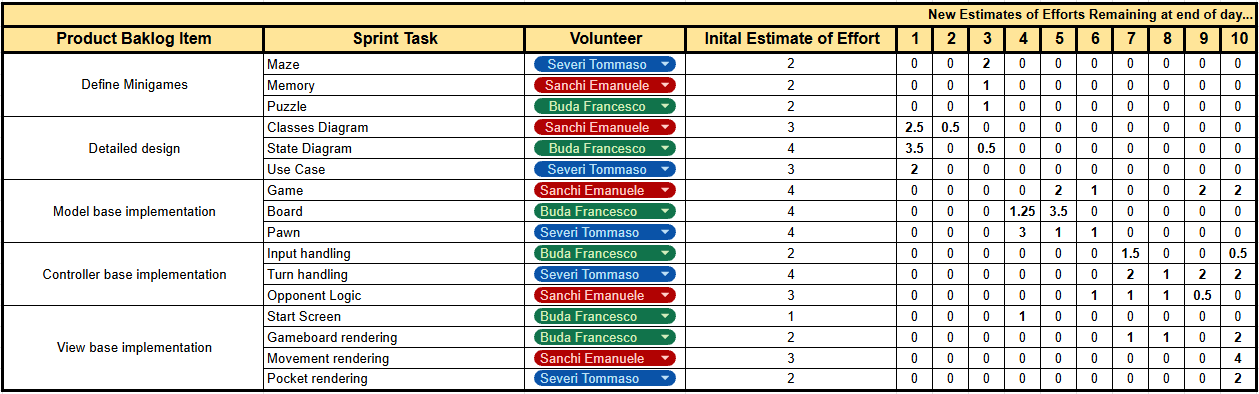
\includegraphics[width=1\textwidth]{figures/backlog-sprint-2.png}
    \caption{Backlog per lo Sprint-2}
    \label{fig:backlog-sprint-2}
\end{figure}